\def\year{2018}\relax
%File: formatting-instruction.tex
\documentclass[letterpaper]{article} %DO NOT CHANGE THIS
\usepackage{aaai18}  %Required
\usepackage{times}  %Required
\usepackage{helvet}  %Required
\usepackage{courier}  %Required
\usepackage{url}  %Required
\usepackage{graphicx}  %Required
\frenchspacing  %Required
\setlength{\pdfpagewidth}{8.5in}  %Required
\setlength{\pdfpageheight}{11in}  %Required
\copyrighttext{Copyright 2017, California Institute of Technology. 
Government sponsorship acknowledged.}
%PDF Info Is Required:
  \pdfinfo{
/Title (Extracting Information from Scientific Publications for
Planetary Science)
/Author (Kiri L. Wagstaff, Raymond Francis, Thamme Gowda, Nina L. Lanza,
You Lu, Ellen Riloff, Karanjeet Singh)}
\setcounter{secnumdepth}{0}  
 \begin{document}
% The file aaai.sty is the style file for AAAI Press 
% proceedings, working notes, and technical reports.
%
\title{Extracting Information from Scientific Publications for
Planetary Science}
\author{
Kiri L. Wagstaff$^1$,
Raymond Francis$^1$,
Thamme Gowda$^{1,2}$,
Nina L. Lanza$^3$,\\
{\Large \bf You Lu$^1$,
Ellen Riloff$^4$, and
Karanjeet Singh$^{1,5}$}\\
$^1$Jet Propulsion Laboratory, California Institute of Technology,
4800 Oak Grove Drive, Pasadena, CA 91109\\
\{firstname.lastname\}@jpl.nasa.gov\\
$^2$Information Sciences Institute, University of Southern
California,
4676 Admiralty Way \#1001, Marina Del Rey, CA 90292\\
tg@isi.edu
}
\maketitle
\begin{abstract}
We have constructed an information extraction system called the Mars
Target Encyclopedia that takes in planetary science publications
and extracts scientific knowledge.  The extracted knowledge is stored
in a searchable database that can greatly accelerate the ability of
scientists to compare new discoveries with what is already known.  To
date, we have applied this system to $\sim$6000 documents and achieved
XX\% precision in the extracted information. 
\end{abstract}

\section{Introduction}

Scientists everywhere are overwhelmed by the stream of new information
that is published by their disciplines' conferences, workshops, and
journals.  It is increasingly difficult to come up to speed in a
new area and to stay current with the latest discoveries.  In
planetary exploration, new discoveries can occur each time
new data is transmitted.  For example, our rovers on Mars have sent
back compositional data for thousands of individual targets (e.g.,
rocks, soils), and some of those observations have transformed our
understanding of past environments on the planet {\bf
[cite... Nature?]}.

To interpret new observations correctly, it is necessary to be able to
compare them with what is already known.  For example, if we observe
high manganese content at a particular location, we want to know
whether it is consistent with previous observations or it indicates an
anomalous new discovery.  However, no central database exists in which
planetary scientists can quickly make that determination.

We have created a system that uses information extraction methods to
analyze planetary science publications and identify compositional
relationships between Mars surface targets and elements or minerals.
The extracted information is stored in a searchable database that
allows users to ask questions such as ``Which targets contain
hematite?'' or ``What is known about target Dillinger?''  It also
enables entirely new kinds of information visualization, such as a map
display of all locations where the Mars rover Curiosity has detected
hematite. 

We focus on the extraction of information about targets identified by
the ChemCam instrument on the Mars Science Laboratory rover.  ChemCam
obtains compositional spectra from up to seven meters away from a
given target, and the resulting spectrum can be analyzed to identify
individual elements within the target~\cite{maurice:chemcam12}.  As of
sol 1159, ChemCam had observed more than 1100 distinct targets.

... provide guidance for next steps in exploration 
- hypothesis generation and data collection.

leveraged a small amount of hand-labeled text to train a

precision more important than recall

\section{Related Work}

GeoDeepDive

work at ISI?

\section{Machine Learning for Information Extraction}

The Mars Target Encyclopedia (MTE) is an information extraction system
that takes in scientific publications in PDF format and extracts
knowledge of use to planetary scientists studying the planet Mars.
The MTE is composed of four modules: preprocessing, named entity
recognition (NER), relation extraction (RE), and database updates (see
Figure~\ref{fig:mte}).

\begin{figure}
\begin{center}
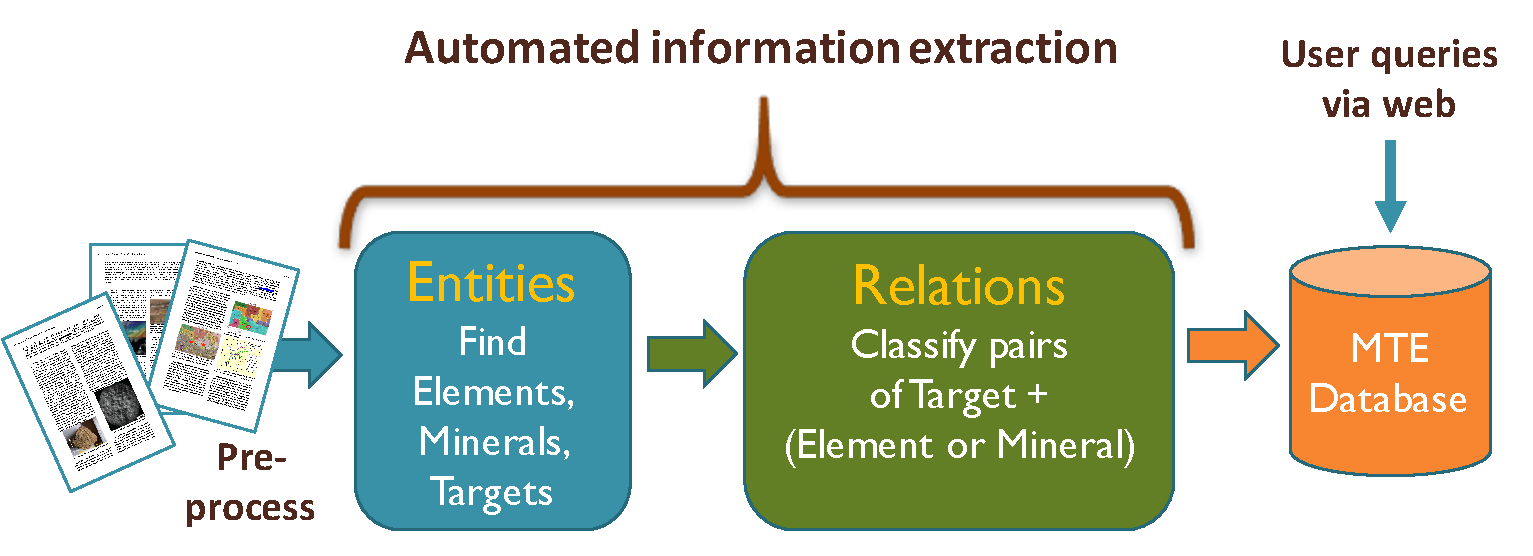
\includegraphics[width=3.25in]{fig/system.pdf}
\end{center}
\caption{Mars Target Encyclopedia processing pipeline.}
\label{fig:mte}
\end{figure}
% This figure comes from 2017-06-23-mte.pptx

\subsection{Document Preprocessing}

To prepare the documents for information extraction, the MTE first
extracts the text content from each PDF document.  We use the Apache
Tika parser~\cite{mattmann:tika11} to convert the source PDF files
into UTF-8 format text to preserve accented characters and
mathematical symbols.
% more details from extract_text_utf8.py?
Next, the MTE creates a copy of the text content in which the
References section is omitted.  We defined a regular expression to
identify the References section.
% show the regexp?
This step helps the NER component avoid spurious detections in the
titles or author names of cited publications.

\subsection{Named Entity Recognition}

The named entities of greatest relevance for the MTE are elements
(e.g., ``iron,'' ``Mg''), minerals (e.g., ``plagioclase,''
``hematite''), and ChemCam targets.  The periodic table provides a
comprehensive list of elements, and we employed a list of 5228
minerals provided by the International Mineralogical Association (the
May 2017 release\footnote{\url{http://nrmima.nrm.se/imalist.htm}}). 

Identifying Mars surface targets is more challenging, as they follow
no standard naming convention.  Further, target names are
fundamentally ambiguous as they are borrowed from Earth locations or
people.  A sampling of the names hints at the challenge of accurately
detecting them: ``Dunkirk'', ``Ithaca'', ``Jake'', ``Old\_woman'',
``Pistol''.  We have a starting list of target
names\footnote{\url{http://pds-geosciences.wustl.edu/msl/msl-m-chemcam-libs-4_5-rdr-v1/mslccm_1xxx/document/msl_ccam_obs.csv}}
that was published by the ChemCam science team, but it is not fully
curated, and we have found it to be incomplete with respect to the
literature.
%
In addition, we found that authors invent new spelling
variants and abbreviations for target names that require more than a
simple list lookup.
% Keyword-based web or publication searches return many spurious hits.

To address the challenge of recognizing all three entity classes
reliably, we employed a machine learning approach.  We trained a
custom Named Entity Recognizer (NER) using the Stanford CoreNLP NER
system~\cite{finkel:ner05}.  This system trains a Conditional Random
Field sequence model to assign class labels to entities within new
documents.  We provided manually labeled documents with examples of
the Element, Mineral, and Target classes to train the our custom
model.  We also employed the ``gazette'' capability to provide lists
of known terms.  This is particularly valuable for large semantic
classes (like Mineral or Target) in which terms exist that might never
appear in the training corpus.  The gazettes we used include the
periodic table (Elements), the IMA list (Minerals), and the ChemCam
observation table (Targets) as mentioned above.

Details:
- CoreNLP data format (inside/outside encoding) - see Steven's wiki
page

{\bf [gazettes are available where online]}

We also employed the Basilisk bootstrapping algorithm to learn
additional related terms that belong to each entity
class~\cite{thelen:basilisk02}.  {\bf [Ellen: add brief blurb about
Basilisk]}  It was our hope that Basilisk, which operates on unlabeled
text, might learn terms that would otherwise escape the CRF
classifier, which can only learn from labeled text.  These could
include author-created abbreviations and alternate spellings.

\subsection{Relation Extraction}

Once the entities are identified witin the text, the MTE analyzes them
to determine which ones have a compositional relationship (i.e.,
textual evidence that a given Target contains a given Element or
Mineral).  
%
We trained a relation classifier using the jSRE~\cite{giuliano:jsre06}
relation extraction tool.  It trains an SVM classifier to predict
whether a relationship exists for two entities, using only shallow
parsing.  jSRE provides SVM kernels that oeprate on local context,
global (sentence-wide) context, or a combination of both.  In applying
this method to biomedical publications, the authors found that most of
the performance came from the global kernel features.

Details:
- jSRE example format encoding
- multi-word tokens should be merged with underscores... instead, we
operated on a per-word basis and merged relations as appropriate (hack)

\section{Experimental Results}

We developed and evaluated the MTE using a collection of scientific
papers that were published over three years of the Lunar and Planetary
Science Conference (LPSC).

\subsection{Corpus}

Our corpus consists of two-page extended LPSC abstracts in PDF format.
We selected 117 documents from LPSC 2015 and 2016 that mentioned
``ChemCam.''  We used the html-based brat annotation tool~\cite{brat}
to manually label entities and relations within these documents.  We
estimate that it took an average of 30 minutes to annotate each
document.  We created thousands of manual annotations in 62 documents
from LPSC 2015 and 55 documents from LPSC 2016 (see
Table~\ref{tab:docs}).

% cut -f2 *.ann | cut -f1 -d' ' | cut -f1 -d':' | sort | uniq -c
\begin{table}
\caption{Manual annotations for LPSC documents.}
\label{tab:docs}
\begin{center}
\begin{tabular}{l|ccc}
           & 2015     & 2016     & Total \\ 
Annotation & (62 docs) & (55 docs) & (117 docs)\\ \hline
Element  & 1195 & 1029 & 2224 \\
Mineral  & 748  & 708  & 1456 \\
Target   & 566  & 347  &  913 \\ \hline
Contains & 434  & 262  &  696 \\ \hline
Total    & 2943 & 2346 & 5289 \\ \hline
\end{tabular}
\end{center}
\end{table}

The annotated relationships ranged from simple (e.g., a pattern such
as ``X contains Y'' within a sentence) to complex (e.g., relationships
that crossed sentence boundaries or involved pronouns like ``it'' and
other anaphora).  Figure~\ref{fig:brat} shows an excerpt from one
document that contains several statements about the composition of the
target Buckskin.  The vocabulary used to indicate a compositional
relationship varies, and the last two relationships cross sentence
boundaries.  

\begin{figure}
\begin{center}
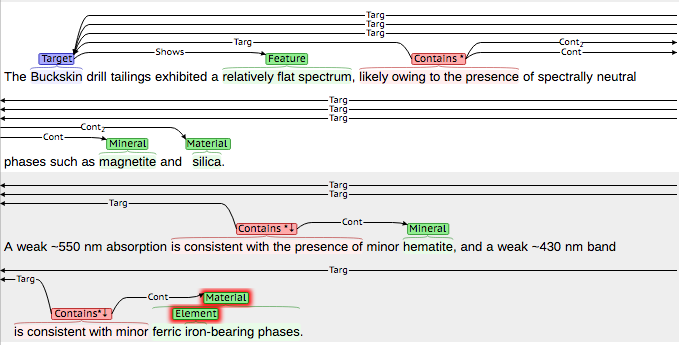
\includegraphics[width=3.25in]{fig/brat-example.png}
\end{center}
\caption{Excerpt from document lpsc16-1155 showing compositional
annotations created with the brat web annotation tool.}
\label{fig:brat}
\end{figure}

{\bf [annotated docs are available where?]}

\subsection{Named Entity Recognition Results}

Named entity recognition operates on individual words or tokens.  We
used the 2015 documents for training and divided the 2016 documents
into validation ($n=20$) and testing ($n=35$) sets.  (Total number of
items?) 

\begin{table}
\caption{Named entity recognition performance on LPSC 2016 test documents.  
The best result is shown in bold.}
\label{tab:ner}
\begin{center}
\begin{tabular}{l|ll}
 & Precision & Recall \\ \hline
Baseline: Random & P & R \\
Baseline: Lists only & P & R \\ \hline
{\em CoreNLP NER CRF trained on:} & & \\
LPSC 2015 & P & R \\
LPSC 2015 + gazettes & 0.944 & 0.777 \\
LPSC 2015 + Basilisk gazettes & P & R \\
\hline
\end{tabular}
\end{center}
\end{table}

{\bf [precision/recall per class - bar plot?]}

Basilisk - output manually reviewed

\subsection{Relation Extraction Results}

The decision about whether or not a relation exists is made for a
given pair of entities.  Processing all possible pairs of entities in
a document would be infeasible (and likely unnecessary).  For
simplicity, we adopted the strategy used in previous
work~\cite{giuliano:jsre06} of generating all pairs of entities that
occur within a single sentence.  We used CoreNLP's sentence splitter
to divide the corpus into sentences and the NER model trained above to
identify entities.  For each (Target, Element) or (Target, Mineral)
pair, we generated a jSRE example that encoded the sentence content.
If the pair of entities was connected by a relation in the manual
annotations, we gave the example a positive label; otherwise, we gave
it a negative label.

To simulate how the system would be used in practice, we trained and
validated the relation classifier using text from LPSC 2015 and tested
it on LPSC 2016.  We used the first 42 LPSC 2015 documents for
training and the remaining 20 for validation.  The number and
distribution of the resulting jSRE examples (relationships) are given
in Table~\ref{tab:rels}.  

% for l in lpsc16-utf8/*test ; do echo $l ; cut -f1 $l | sort | uniq -c; done
\begin{table}
\caption{Number and distribution of relationships between Targets and
Elements or Minerals. The number in parentheses is the percentage of
positive relationships. }
\label{tab:rels}
\begin{center}
\begin{tabular}{l|ccc}
           & Element & Mineral & Merged \\ \hline 
Train      & 279 (38\%) & 150 (41\%) & 429 (39\%) \\
Validation &  93 (27\%) &  70 (69\%) & 163 (45\%) \\ \hline
Test       & 111 (37\%) &  62 (50\%) & 173 (42\%) \\ \hline
\end{tabular}
\end{center}
\end{table}

We trained three different relation classifiers: one on Target-Element
relations only; one on Target-Mineral relations only; and one on the
merged set.  We were curious as to how a specialized model that was
trained on less data would compare to a more generic model trained on
more data.  For each model, we performed a grid search over the jSRE
parameters by trying each of the SVM kernels (LC, GC, SL) and window
sizes within the set \{ 1, 2, 5, 10, 15, 20 \}.  We selected the model
parameters that led to the highest performance on the validation set
in terms of precision.

We found that the merged model out-performed the specialized models by
a large margin (see Table~\ref{tab:re}).  We also found that the
max-precision model did not employ the same parameters across the
three models.  Target-Element and Target-Merged used an LC kernel with
a window of 5, while Target-Mineral used an SL kernel with a window of 5.

\begin{table}
\caption{Relation extraction performance on LPSC 2016 documents. 
The highest-precision result for each data set is shown in bold.}
\label{tab:re}
\begin{center}
\begin{tabular}{l|ll}
 & Precision & Recall \\ \hline
%{\em jSRE SVM trained on:} & & \\
\multicolumn{3}{c}{Elements ($n=111$)} \\
jSRE-Elements & {\bf 0.531} & 0.415 \\
Baseline: All-yes & 0.369 & 1.000 \\ \hline
\multicolumn{3}{c}{Minerals ($n=62$)} \\
jSRE-Minerals & {\bf 0.679} & 0.613 \\ 
Baseline: All-yes & 0.500 & 1.000 \\ \hline
\multicolumn{3}{c}{Merged ($n=173$)} \\
jSRE-Merged  & {\bf 0.640} & 0.444 \\
jSRE-Indiv.  & 0.598 & 0.447 \\
Baseline: All-yes & 0.416 & 1.000 \\ \hline
\end{tabular}
\end{center}
\end{table}

We also compared the models to a baseline approach that always
predicted that a relationship was present (``All-yes'').  While this
baseline always achieves a recall of 1.00, its precision is much lower
than that of the jSRE classifier.

Also:
- mineral is an easier problem than element?
- these are separate evaluations because separate data sets
- recall is somewhat low, but precision is far more important

{\bf [precision/recall per class - bar plot?] }

\subsection{Large-scale Evaluation}

We collected all 6000 {\bf [check]} LPSC documents that were published
in 2014, 2015, and 2016 and ingested them into the MTE.  This large
corpus contains the 117 documents used for development and evaluation
as well as everything else that was published at these conferences.

{\bf [table of num docs, num NER, num RE, time consumed]}

{\bf [Nina's evaluation of extracted information]}

{\bf [spatial map - hematite search - where does this fit?]}

\subsection{Limitations}
- NER cannot handle overlapping annotations (e.g., calcium sulfate)
- RE: no sentence-crossing relationships (about 30\%? recalc this
  number, restrict to element/mineral (no material))

\section{Conclusions and Next Steps}
% and lessons learned

This work lies at the intersection of information extraction, machine
learning, and planetary science.  

% or is this a limitation (prev section)?
The MTE is not comprehensive.  There may be compositional information
that was never written up in a scientific publication and therefore
would not be included in the MTE.  Instead, the MTE extracts and
indexes only the information that was judged by scientists to be
worthy of publication to the scientific community.  The MTE leverages
and mirrors this selection bias, and its holdings (like the source
publications) contain only the most valuable and salient information.

We are in the process of integrating the MTE's content into the MSL
Analyst's Notebook, an interactive web resource for mission scientists
and the interested public.  The Analyst's Notebook allows users to
browse mission plans, targets discovered, data collected, and
summaries of each mission day on Mars.  The MTE content will enable
the Analyst's Notebook to also connect targets to publications.

Expand to targets identified by other missions such as the Mars
Exploration Rovers (Spirit and Opportunity).

\section{Acknowledgments}
This research was carried out in part at the Jet Propulsion Laboratory,
California Institute of Technology, under a contract with the National
Aeronautics and Space Administration.  {\bf [acks for Ellen, Nina?]}

\bibliography{mte}
\bibliographystyle{aaai}
\end{document}
